\documentclass[letter,11pt]{article}

\usepackage{amsfonts}
\usepackage{amsmath}
\usepackage{amssymb}
\usepackage[brazilian]{babel}
\usepackage{enumerate}
\usepackage[T1]{fontenc}
%\usepackage[ansinew,latin1]{inputenc}
\usepackage[utf8x]{inputenc}
\usepackage{multicol}
\setlength\columnseprule{0.5pt}

\newtheorem{exer}{Exercício}
\newtheorem{teo}{Teorema}

\newcommand{\var}{Var}
\newcommand{\E}{\mathbb{E}}

\newcommand{\mat}[1]{\mbox{\boldmath{$#1$}}}

\usepackage[letterpaper,top=3cm, bottom=2cm, left=2.5cm, right=2.5cm]{geometry}

\begin{document}

%\thispagestyle{empty}
\begin{center}{ \Large MAT02026 - Inferência B }\end{center}

\begin{center}
{\large  \sc Gabarito Lista 2}
\end{center}
\vspace{5mm}

%%%%%%%%%%%%%%%%%%%%%%%%%%%%%%%%%%%%%%%%%%%%%%%%%%%%%%%%%%%%%%%%%%%%%%%%%%%%%%%
\begin{exer} \rm
% O que é uma quantidade pivotal? Exemplifique.
\end{exer}


\begin{exer} \rm
% A afirmação: ``Há 95\% de probabilidade do parâmetro $\theta$ estar contido no intervalo $[0,3 ; 0,35]$" está correta? Justifique.
% \end{exer}
% 
% \begin{exer} \rm
% Seja $X_1, \ldots, X_n \sim N(\mu, \sigma^2)$, indique uma quantidade pivotal para:
% 
% \begin{enumerate}[a)] 
% 
% \item $\mu$, com variância conhecida;
% 
% \item $\mu$, com variância desconhecida;
% 
% \item $\sigma^2$.
% 
% \end{enumerate}
\end{exer}


\begin{exer} \rm
 % Sabe-se que em indivíduos hipertensos a pressão distólica pode ser considerada com uma variável que apresenta distribuição normal com os parâmetros $\mu$ e $\sigma^2$ (ambos   desconhecidos). Uma amostra aleatória de 12 hipertensos é selecionada apresentando média de 135mmHg e s=2,4495mmHg. Encontre um intervalo com 90\% de confiança para a média populacional e para a variância populacional. Interprete os resultados.
\end{exer}


\begin{exer} \rm
 % Um experimento foi conduzido para verificar se uma moeda é honesta. O experimento consistiu em arremessar esta moeda e observar o resultado. Foram observadas 179 caras em uma amostra aleatória de 400 arremessos. Encontre um IC com 99\% para $\theta$ (probabilidade de cara). Interprete o resultado encontrado,  a moeda parece ser honesta?
\end{exer}


%Exercicio Marcio - arquivo '02Lista2_Marcio.tex'
\begin{exer} \rm
% Na construção de intervalos de confiança para a proporção $p$ (ou parâmetro $p$ de uma distribuição Bernoulli) podemos utilizar diferentes métodos como descrito no `Plano Aula 4' (arquivo `InferenciaB\_aula4\_topicos.pdf'). Use o R para gerar amostras ($n=10$ e depois $n=100$) Bernoulli para um determinado parâmetro p (digamos $p=0.2$) e construa os Intervalos de Confiança com coeficiente de confiança $(1-\alpha)100\%$ utilizando os três métodos. Sabe-se que ao repetir o experimento é esperado que os intervalos contenham o parâmetro em $(1-\alpha)100\%$ das vezes. Então fixe $\alpha =0.05$, repita o experimento 1000 vezes para os três métodos e verifique se em 95\% das vezes o intervalo contém o parâmetro $p=0.2$. Qual sua conclusão? Os intervalos possuem mesmo a confiança desejada?
% 
% \noindent (Obs.: Também é possível utilizar o método \textit{bootstrap} paramétrico, comentado no 'Plano Aula 5'.)
\end{exer}


\begin{exer} \rm
 % Por que $H_1$ é chamada de hipótese de pesquisa?
\end{exer}


\begin{exer} \rm
 % Quais os tipos de erros de um teste de hipóteses? Utilize um exemplo e indique quais os erros possíveis que um pesquisador pode cometer ao fazer um teste de hipóteses.
\end{exer}


\begin{exer} \rm
 % Qual o comportamento da função poder ideal?
\end{exer}


\begin{exer} \rm
 % Explique com suas palavras qual a idéia do TRV.
\end{exer}


\begin{exer} \rm
 % Explique com suas palavras o que é um teste de hipóteses.
\end{exer}


\begin{exer} \rm
 % Explique com suas palavras o que é um intervalo de confiança.
\end{exer}

\begin{exer} \rm
 % Explique com suas palavras o que é um intervalo de confiança.
\end{exer}

% Exercício Marcio - exercicio_para_entregar1.tex
\begin{exer} \rm
% Seja $X\in\{1,2,3,4\}$ uma variável aleatória com função massa de probabilidade $P_\theta(X=k)$, para $\theta\in\Theta=\{0,1\}$ e $k\in\{1,2,3,4\}$ dada pela seguinte tabela
\begin{enumerate}[a)] 
  \item %Considere o teste A que rejeita $H_0$ se $X \leq 2$ e o teste B que rejeita $H_0$ se $X$ é par. 
  %Calcule as probabilidades $\alpha$ e $\beta$ para ambos os testes.
  Parcialmente feito em aula.
  \item %Use o Lema de Neyman-Pearson para encontrar o teste MP para um nível de significancia de 5\%.

\begin{center}
\begin{tabular}{c|cccc}
& $P_\theta(X=1)$ & $P_\theta(X=2)$ & $P_\theta(X=3)$ & $P_\theta(X=4)$ \\
\hline
$\frac{L_1}{L_0}$ & 5 & 10 & 10 & 0.43 \\
\end{tabular}
\end{center}
Pelo Lema NP calculamos $L_1 / L_0$ e verificamos (não está tão claro aqui) que há indício de que para valores pequenos de $X$ maior a evidência de $H_1$ em relação a $H_0$ (maior a razão $L_1/L_0$). Nesse caso, encontrar uma região crítica do tipo $A_1 = \left\{x: a < x < b \right\}$ tal que $P(a \leq X \leq  b \vert \theta = \theta_1) = 0,05$ são UMP, por exemplo, qualquer valor de $k$ entre 5 e 10 representaria a região $A_1 = \left\{2, 3 \right\}$.

\end{enumerate}
\end{exer}


% Continuacao lista 2 Marcia
\begin{exer} \rm
 Faça os seguintes exercícios do livro Statistical Inference: 

\begin{enumerate}[a)] 

\item %8.1 

\item 8.2 - Seja $X \sim Poisson(\lambda)$ and assuma $X=10$ observado, então 
$$P(X \leq 10 \vert \lambda = 15) = \sum_{i=0}^{10} \frac{\epsilon^{-15} 15^i}{i!} \approx 0,1185$$
O que podemos interpretar a partir dessa probabilidade?

\item %8.4

\item %8.5 (a) e (b)

\item %8.6 (a)

\item %8.7 (b)

\item %8.12

\item %8.13 (a) e (b)

\item %8.14

\item 8.15 - A partir do Lema de Neyman-Pearson temos que a região do teste UMP é dada por $A_1 = \{ \boldsymbol{x}: L_1(\theta) / L_0(\theta) > k \}$ e 
$$ \frac{f(\boldsymbol{x}; \sigma_1)}{f(\boldsymbol{x}; \sigma_0)} =  \frac{ (2 \pi \sigma_1)^{-n/2} \exp 
\left\{ - \frac{\sum_{i=1}^n x_i^2}{2 \sigma_1} \right\} }{ (2 \pi \sigma_0)^{-n/2} \exp 
\left\{ - \frac{\sum_{i=1}^n x_i^2}{2 \sigma_0} \right\}  } = \ldots = \left( \frac{\sigma_0}{\sigma_1} \right)^n \exp \left\{ \frac{1}{2} \sum_{i=1}^n x_i^2  \left( \frac{1}{\sigma_0^2} - \frac{1}{ 
\sigma_1^2} \right) \right\}, \text{ para algum } K \geq 0 .$$
Podemos reescrever a desigualdade acima tal que 
$$ \sum_{i=1}^n x_i^2 > \frac{2 \log \left( k (\sigma_1 / \sigma_0)^n \right)}{\left( \frac{1}{\sigma_0^2} - 
\frac{1}{\sigma_1^2} \right)} = c \hspace{1cm} \left( \text{ use o fato de que } \left( \frac{1}{\sigma_0^2} - \frac{1}{\sigma_1^2} \right) \right).$$
Ainda, o Lema de Neyman-Pearson diz que o test UMP de tamanho $\alpha$ satisfaz 
$\alpha = P \left( \sum_{i=1}^n X_i^2 > c \vert \sigma = \sigma_0 \right)$.
Como obter $c$? (Sob $H_0$ supomos $\sigma = \sigma_0$ e) sabemos que $Q(\boldsymbol{X}) = \sum_{i=1}^n X_i^2 / \sigma_0^2 
\sim \chi^2_n$ (porquê?), então
$$\alpha = P_{\sigma_0} \left( \sum_{i=1}^n X_i^2 >  c \right) = P_{\sigma_0} \left( \sum_{i=1}^n \frac{ 
X_i^2 }{\sigma_0^2} >  \frac{ c }{\sigma_0^2} \right) = P_{\sigma_0} \left( Q >  \frac{ c }{\sigma_0^2} \right).$$
Por fim, denote $q_{n; \alpha}$ tal que $P(Q < q_{n; \alpha}) = \alpha$, assim $\frac{c}{\sigma^2_0} = q_{n; \alpha} \Leftrightarrow c = \sigma^2_0 \times q_{n; \alpha}$.
% \begin{figure}
% 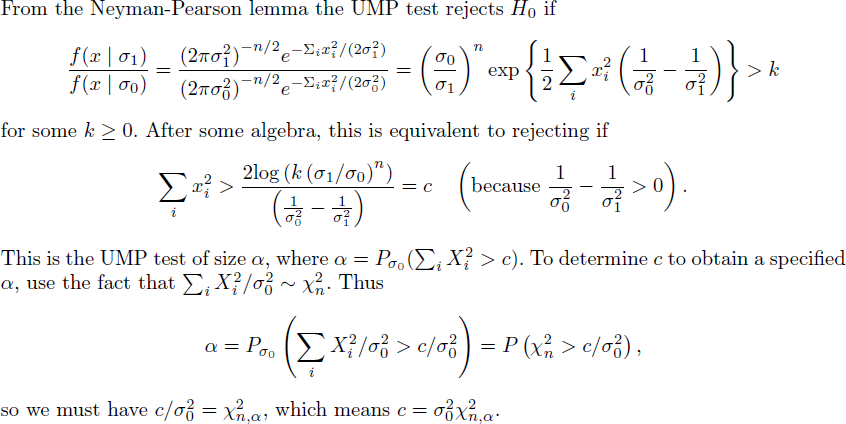
\includegraphics[scale=0.7]{Ex8_15CasellaBerger.jpg}
% \end{figure}

\item %8.16

\item %8.17 (a) e (b)

\item %8.18

\item %8.19

\item %8.20

\item %8.21

\clearpage
\item 8.22 (a) O Lema de Neyman-Pearson nos diz que a região de rejeição do teste UMP de tamanho $\alpha$ é dada por $L_1 / L_0 > k$. Mostre que o lema nos leva a uma região crítica do tipo $A_1^* = \left\{ \sum_{i=1}^10 X_i < c \right\}$. Temos que $Y = \sum_{i=1}^10 X_i \sim Binomial(10, p)$ e denote sua p.m.f. $f(\boldsymbol{x}; p)$. A tabela abaixo mostra as distribuições sob $H_0$, $H_1$ e a razão entre as distribuições (verossimilhanças). Note que valores grandes de $L_1 / L_0$ significam pequenos valores de $Y=y$.

\begin{table}[hh]
  \begin{tabular}{cccccccccccc}
    \hline
    $y$ & 0 & 1 & 2 & 3 & 4 & 5 & 6 & 7 & 8 & 9 & 10 \\
    \hline
    $f(y; 1/2)$ & 0,00 & 0,01 & 0,04 & 0,12 & 0,21 & 0,25 & 0,21 & 0,12 & 0,04 & 0,01 & 0,00 \\
    $f(y; 1/4)$ & 0,06 & 0,19 & 0,28 & 0,25 & 0,15 & 0,06 & 0,02 & 0,00 & 0,00 & 0,00 & 0,00 \\
    $\frac{f(y; 1/4)}{f(y; 1/2)}$ & 57,67 & 19,22 & 6,41 & 2,14 & 0,71 & 0,24 & 0,08 & 0,03 & 0,01 & 0,00 & 0,00 \\
    \hline
  \end{tabular}
\end{table}
Então, para o teste de tamanho $\alpha = 0,0547$ precisamos encontrar $c$ tal que $ 0,0547 = P(Y \leq c \vert p=1/2)$. Por fim, olhando a tabela acima, verifique que $P(Y \leq 2 \vert p=1/2) = 0,0547$, assim a região crítica do teste UMP com tamanho $\alpha = 0,0547$ é dada por $A_1 = \left\{ {\sum_{i=1}^10 \leq 2 \right\}$. O poder do teste é dado por $\pi(p_1) = 1 - \beta = P(Y \geq 2 \vert p=1/4) \apporx 0,526$
% p0 <- dbinom(0:10, 10, 1/2)
% p1 <- dbinom(0:10, 10, 1/4)
% round(rbind(0:10, p0, p1, p1/p0), 2)

\item 8.23 (b) Utilizando-se o Lema de Neyman-Pearson temos que o teste MP nesse caso tem região de rejeição do tipo $f(x; \theta=2) / f(x; \theta=1) > k$ para algum $k \geq 0$. Usando a f.d.p. da distribuição Beta temos
$$ \frac{f(x; \theta=2)}{f(x; \theta=1)} = \frac{ \frac{ \Gamma(2+1) }{ \Gamma(2) \Gamma(1) } x^{2-1} (1-x)^{1-1}}{\frac{ \Gamma(1+1) }{ \Gamma(1) \Gamma(1) } x^{1-1} (1-x)^{1-1}} = 2x.$$
Assim o teste MP tem região de rejeição $A_1^* = \{ x: x > k/2 \}$. Para encontrar $k$, o Lema diz que o teste de tamanho $\alpha$ satisfaz 
$$ \alpha = P(X > k/2 \vert \theta = 1) = \int_{k/2}^{1} \frac{\Gamma(1+1)}{\Gamma(1)\Gamma(1)} x^{1-1} (1-x)^{1-1} dx = 1 - \frac{k}{2}.$$
Então, temos que $\alpha = 1-\frac{k}{2}$ e o teste UMP tem região de rejeição $A_1^* = \{ x: x > 2(1-\alpha)/2 \} = \{ x: x > 1-\alpha \}$. 

\item %8.24

\end{enumerate}
\end{exer}

%% Exercicios da lista 1 Marcia... incluir???
% \begin{exer} \rm
% Suponha que a proporção $p$ de itens defeituosos, em uma grande população de itens, 
% seja desconhecida. Deseja-se testar as seguintes hipóteses $H_0 : p = 0,2$ versus 
% $H_1 : p \neq 0,2$. Considere que uma amostra aleatória de 20 itens seja retirada 
% desta população e denote $Y$ = número de itens defeituosos na amostra. O seguinte 
% procedimento de teste será usado: Rejeitar $H_0$ se $Y \geq 7$ ou $Y \leq 1$.
% \begin{enumerate}[a)]
%   \item Determine a funcão poder deste teste.
%   \item Calcule o valor da função poder para os seguintes pontos 
%   $p = \{0, 0.1, 0.2, 0.3, 0.4, 0.5, 0.6, 0.7, 0.8, 0.9, 1\}$. Faça o gráfico.
%   \item Determine o tamanho do teste, ou seja, o valor de $\alpha = \sup_{\theta 
%   \in\Theta_0} \beta(\theta)$.
% \end{enumerate}
% \end{exer}
% 
% 
% \begin{exer} \rm
% Seja $X_1, \ldots, X_{10} $ uma amostra aleatória de tamanho $n = 10$ tal que 
% $X_i \sim Bernoulli(\theta)$ onde $P(X_i = 1) = \theta = 1 - P(X_i = 0)$. 
% Considere as hipóteses $H_0 : \theta \leq 1/2$ contra $H_1 : \theta > 1/2$. 
% Assuma a seguinte regra de teste: Rejeitar $H_0$ se $\sum X_i \geq 6$.
% \begin{enumerate}[a)]
%   \item Determine a função poder do teste.
%   \item Calcule a função poder para os seguintes pontos $p = \{0, 0.1, 0.2, 0.3, 0.4, 0.5, 0.6, 0.7, 0.8, 0.9, 1\}$. Faça o gráfico.
%   \item Determine o tamanho do teste, ou seja, o valor de $\alpha = \sup_{\theta \in\Theta_0} \beta(\theta)$.
% \end{enumerate}
% \end{exer}
% 
% 
% \begin{exer} \rm
% Considere a variável aleatória $X$ com a seguinte densidade $f(x) = \theta x^{\theta-1}I_{(0,1)}(x)$. Para testar as hipóteses $H_0 : \theta \leq 1$ versus $H_1: \theta > 1$, uma única observação $(X_1)$ foi amostrada e o seguinte critério de rejeição foi adotado: rejeitar $H_0$ se $X_1 > 1/2$.
% \begin{enumerate}[a)]
%   \item Encontre a função poder deste teste.
%   \item Determine o tamanho do teste.
% \end{enumerate}
% \end{exer}

\end{document}